\documentclass[10pt,journal,compsoc]{IEEEtran}

\usepackage{amsmath,amssymb,amsfonts}
\usepackage{algorithmic}
\usepackage{graphicx}
\usepackage{textcomp}
\usepackage{xcolor}
\usepackage{booktabs}
\usepackage{tabularx}
\usepackage{hyperref}
\usepackage{tikz}
\usetikzlibrary{arrows.meta,positioning,shapes.geometric,calc}

\hypersetup{
    colorlinks=true,
    linkcolor=blue,
    filecolor=magenta,      
    urlcolor=cyan,
    citecolor=blue
}

\begin{document}

\title{Multi-Objective Visual Attention for Traffic Camera Feeds}

\author{Rei Tamaru
\thanks{Manuscript finalized September 2026. Document describes running system specifications and baseline empirical evaluations.}}

% \markboth{}%
% {Prioritizing Traffic Camera Feeds with Multi-Objective Visual Attention}

\IEEEtitleabstractindextext{%
\begin{abstract}
Video walls in traffic management centers can show only a few of the camera feeds available to them. Ranking feeds by frame motion alone fails because the amount of motion in a picture does not rise with its operational importance. A blockage across several lanes can leave a picture still, while free-flowing rush-hour traffic changes from frame to frame as much as any picture can. This paper presents \textbf{rt511}, an open-source system that ranks public traffic camera feeds for a display wall. A continuous scorer combines an hour-of-week anomaly estimate with empirical Bayes shrinkage, a road-size amplifier and lexicographic consequence floors raised by incident records and by queues carried upstream along a directed road graph. An episodic language-model arbiter is consulted only for cases the arithmetic cannot settle, and its answers pass confidence gates before they change any score. The system indexes 7,394 cameras from five agency feeds in seven states. A synthetic benchmark of five scripted scenarios, run over 30 seeds at four picture rates, shows the rules surfacing an unusual street at a quiet hour, an unusual arterial at rush hour and a reported crash with its upstream queue, and failing to surface stopped traffic unless a standstill is confirmed. A live trace of one city found that routine maintenance records held every prominent place on the wall, a fault removed by excluding planned work from the floors. Both are specification tests and observations of the rules, not measures of how well the ranking matches human attention.
\end{abstract}

\begin{IEEEkeywords}
Intelligent Transportation Systems, Information Foraging Theory, Kinematic Wave Theory, Multimodal Reasoning.
\end{IEEEkeywords} }

\maketitle
\IEEEdisplaynontitleabstractindextext
\IEEEpeerreviewmaketitle

\section{Introduction and Problem Formulation}
\IEEEPARstart{M}{onitoring} regional highway and arterial closed-circuit television (CCTV) grids presents a severe cognitive overload and an acute human visual foveation bottleneck \cite{pirolli1999}. Advanced Traffic Management Centers (TMCs) routinely manage thousands of simultaneous camera streams, producing an aggregate visual bandwidth that vastly outstrips the perceptual and attentional capacity of human operators \cite{itti1998}. Conventional video wall scheduling paradigms rely primarily on static round-robin rotation cycles or uncalibrated frame-differencing motion thresholds \cite{itti1998}. 

These naive allocation strategies break down under the non-monotonic dynamics of traffic flow \cite{greenshields1935}. In particular, unconstrained free-flow rush-hour movement generates continuous pixel variance that monopolizes motion-sensitive salience models without representing actionable operational disruption \cite{itti1998}. Conversely, acute bottleneck formations, such as multi-lane blockages or severe incident queues, frequently exhibit near-zero inter-frame pixel differences, causing conventional motion-driven systems to erroneously demote critical hazards to minimal visual prominence \cite{lighthill1955, richards1956}.

To overcome this structural failure, we present \textbf{rt511}, an open-source visual attention orchestration system that frames large-scale surveillance scheduling as a multi-objective optimization problem \cite{pirolli1999}. The system decouples visual attention into three orthogonal axes: Anomaly (Bayesian surprise relative to diurnal history), Spectacle (bottom-up kinetic salience), and Consequence (lexicographically ordered operational risk) \cite{fishburn1974, itti2009}. By formulating incident consequence as an invariant mathematical floor rather than an additive weight, severe roadway hazards remain anchored on the physical display regardless of frame stillness \cite{fishburn1974}. A continuous fast-path engine computes network-wide kinematic wave queue propagation, while an episodic reasoning tier (the JEV Arbiter) is consulted on zero-motion edge cases that the arithmetic cannot settle \cite{lighthill1955}. Furthermore, an embedded active-learning module fits an in-browser Bradley--Terry preference model \cite{bradley1952}, projecting empirical operator choices directly into the scoring parameter space to enable continuous alignment and auditing \cite{thurstone1927}.

\section{Theoretical Grounding}
Each mathematical component within \texttt{rt511} is grounded in established cognitive ergonomics, decision theory, and macroscopic traffic flow literature \cite{charnov1976, fishburn1974, lighthill1955, pirolli1999}.

\subsection{Information Foraging Theory and Display Allocation}
We formulate supervisory video surveillance through the lens of Information Foraging Theory (IFT) \cite{pirolli1999}. Under this cognitive model, a human operator functions as an optimal informational forager seeking actionable operational cues (e.g., secondary collisions, unverified queues, hazardous debris) across discrete information patches (individual camera feeds) \cite{pirolli1999}. The composite attention score $S_i(t) \in [0, 1]$ serves as dynamic \textit{information scent}, projecting proximate cues that guide visual traversal and minimize between-patch search costs prior to deep visual consumption \cite{pirolli1999}.

To manage screen real estate without inducing cognitive thrashing, the display allocator operationalizes Charnov's Marginal Value Theorem (MVT) \cite{charnov1976}. High-frequency ranking volatility caused by sensor noise or marginal score fluctuations induces visual fatigue and disrupts situational awareness \cite{charnov1976}. The system introduces a four-rank hysteresis barrier, enforcing an explicit switching-cost penalty: an active feed surrenders its screen tile only when an incoming candidate's information scent exceeds the incumbent's score by a margin sufficient to offset the cognitive reorientation cost of the operator \cite{charnov1976, pirolli1999}.

\subsection{Salience, Surprise, and Exposure Modeling}

The visual prioritization formulation decouples stimulus-driven kinetic salience (Spectacle) from expectation-driven cognitive surprise (Anomaly) \cite{itti1998, itti2009}. While instantaneous inter-frame differencing measures low-level temporal excitation, the anomaly term operationalizes Bayesian surprise \cite{itti2009} by quantifying statistical divergence from a learned diurnal baseline distribution. Furthermore, to account for operational consequence, the system incorporates exposure theory as codified in the \textit{Highway Safety Manual} \cite{aashto2010}: raw visual scores are modulated by Annual Average Daily Traffic (AADT), weighting candidate alerts proportionally to corridor vehicular throughput and network criticality.

\subsection{Macroscopic Flow Duality and Kinematic Wave Shockwave Propagation}
Under Greenshields' parabolic fundamental diagram of traffic flow, the relationship between macroscopic vehicular flow $q$ and density $k$ yields identical boundary conditions $\lim_{k \to 0} q(k) = \lim_{k \to k_j} q(k) = 0$, where $k_j$ denotes jam density \cite{greenshields1935}. Because low-level temporal frame differencing acts as an empirical proxy for visual flow, it inherently inherits this structural singularity, rendering unforced free-flow starvation and severe queue formation indistinguishable based on inter-frame variance alone. To model spatial spillback and anticipate congestion formation upstream of active bottlenecks, rt511 operationalizes the Lighthill--Whitham--Richards (LWR) kinematic wave theory \cite{lighthill1955, richards1956}. When a roadway closure or confirmed standstill occurs, consequence priority floors propagate backward along directed topological links at a parameterized backward-forming shockwave velocity ($v_{\text{wave}} = 15\text{ km/h}$). This formulation establishes a physical, flow-constrained spreading activation mechanism over the roadway graph, prioritizing upstream viewpoints in accordance with the spatial trajectory of the advancing queue tail \cite{collins1975, lighthill1955}.   

\section{Related Work}
\label{sec:related}
The search behind this section was not exhaustive, and a systematic search of transportation and engineering databases for the prioritization of traffic management center cameras is still to be done. The work closest to rt511 falls into five areas.

\subsection{Scheduling Cameras for Scarce Viewing}
Camera scheduling has been studied mainly for active pan-tilt-zoom cameras serving many targets, as in the observation scheduling of Costello et al. \cite{costello2004} and the virtual-vision scheduling of Qureshi and Terzopoulos \cite{qureshi2006}. In the traffic domain, Li et al. \cite{li2024} decide where tilting traffic cameras should point using a graph-based predictor learned online. rt511 shares the premise of scarce viewing capacity but steers no camera, and instead ranks fixed public feeds for a person's display. Field observation of a road traffic control room by Starke et al. \cite{starke2017} describes how operators divide their visual attention across displays, which is the condition rt511 is designed around.

\subsection{Detecting Incidents and Anomalies in Traffic Video}
Video-based incident detection has a long history, from tracking-based accident detection at intersections \cite{kamijo2000} to the study of false alarms from shadows, weather and lighting in deployed systems \cite{shehata2008}. Santhosh et al. \cite{santhosh2021} survey anomaly detection in road surveillance video, the AI City Challenge benchmarks the detection of crashes and stalled vehicles in Iowa DOT video \cite{naphade2021}, and Mandal et al. \cite{mandal2020} apply detection and tracking to DOT camera feeds to reduce manual monitoring. These methods produce detections or alerts. rt511 produces a ranking, works from still pictures a minute or more apart rather than continuous video, and could take any such detector's output as an additional floor.

\subsection{Selecting Views Among Many Cameras}
Multi-camera surveillance has studied which camera to show, surveyed by Natarajan et al. \cite{natarajan2015}. Daniyal et al. \cite{daniyal2010} score each camera's content and select the most informative view of a shared scene, and Daniyal and Cavallaro \cite{daniyal2011} treat the choice as a sequential decision that penalizes switching between cameras, a counterpart to the hysteresis of rt511. These methods choose among views of one scene, while rt511 ranks many cameras on separate roads and weights them by the consequence of what happens there.

\subsection{Attention Allocation in Supervisory Monitoring}
Senders \cite{senders1964} proposed that an observer should sample each channel in proportion to how fast its information changes, and the SEEV model of Wickens et al. \cite{wickens2003} predicts where attention goes from salience, effort, expectancy and value. The terms of rt511 correspond roughly to that model, with anomaly as salience, the hour-of-week baseline as expectancy, and road size and consequence floors as value. SEEV describes where attention goes, while rt511 uses the same ingredients to propose where it should go. Stainer et al. \cite{stainer2013} found that operators of live CCTV spent most of their time on a few spot monitors and chose what to show from expectations about the time of day, which bears on both the hour-of-week baseline and the small number of prominent tiles.

\subsection{Language Models as Rerankers}
Large language models have been used to rerank candidate lists, both listwise \cite{sun2023} and by pairwise comparison \cite{qin2024}. The confidence they state can be better calibrated than their token probabilities \cite{tian2023}, which bears on the gates used here. The second look of rt511 is a listwise rerank of the leading cameras from text descriptions, bounded so that it can move movement but never consequence.

Each component of rt511 therefore has precedent. What has not been found in the work above is their combination for ranking fixed public traffic feeds on a wall. The combination comprises a per-camera hour-of-week baseline over picture differences, exposure weighting, lexicographic consequence floors from incident records and from queues propagated upstream along a road graph, a language model consulted only for cases the arithmetic cannot settle, and a preference model learned from one person's choices. That combination, and the framing of a traffic camera wall as an attention allocation problem, is the contribution of this paper, subject to the fuller search noted above.

\section{System Architecture and Ingestion Pipeline}
The system architecture decouples static, compute-intensive spatial graph generation from high-throughput, low-latency runtime scoring and display coordination. As delineated in Fig.~\ref{fig:architecture}, the pipeline separates offline topology synthesis from the continuous asynchronous execution loop.

\begin{figure}[!t]
\centering
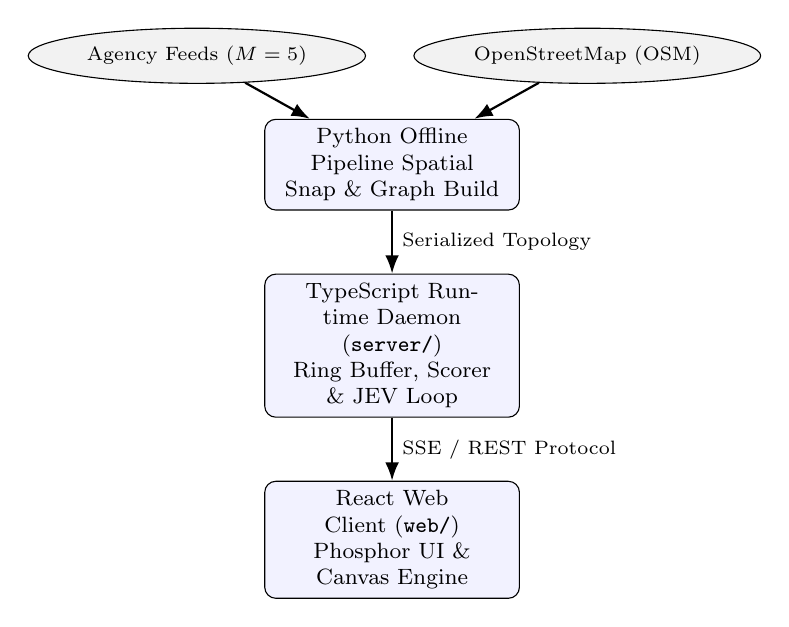
\begin{tikzpicture}[
    node distance=1.1cm and 0.8cm,
    block/.style={rectangle, draw, fill=blue!5, text width=3.0cm, text centered, rounded corners, minimum height=0.9cm, font=\footnotesize},
    cloud/.style={draw, ellipse, fill=gray!10, text centered, minimum height=0.7cm, font=\scriptsize},
    arrow/.style={-Latex, thick}
]
    \node [cloud] (feeds) {Agency Feeds ($M=5$)};
    \node [cloud, right=0.6cm of feeds] (osm) {OpenStreetMap (OSM)};
    \node [block, below=0.8cm of $(feeds)!0.5!(osm)$] (python) {Python Offline Pipeline Spatial Snap \& Graph Build};
    \node [block, below=0.8cm of python] (server) {TypeScript Runtime Daemon\\(\texttt{server/})\\Ring Buffer, Scorer \& JEV Loop};
    \node [block, below=0.8cm of server] (web) {React Web Client (\texttt{web/})\\Phosphor UI \& Canvas Engine};

    \draw [arrow] (feeds) -- (python);
    \draw [arrow] (osm) -- (python);
    \draw [arrow] (python) -- node[right, font=\scriptsize] {Serialized Topology} (server);
    \draw [arrow] (server) -- node[right, font=\scriptsize] {SSE / REST Protocol} (web);
\end{tikzpicture}
\caption{Decoupled subsystem coordination across data boundaries. Offline topological preprocessing ensures zero geometric computation overhead during online stream evaluation.}
\label{fig:architecture}
\end{figure}

\subsection{Data Hygiene and Architectural Invariants}
Operating automated ingestion across public infrastructure necessitates stringent ethical boundaries and data hygiene protocols. The ingestion daemon satisfies three non-negotiable operational invariants:

\begin{itemize}
    \item \textbf{Direct Edge Session Negotiation:} High-bandwidth video transport bypasses the intermediate daemon completely. When an operator selects an active feed, client viewports negotiate direct HTTP Live Streaming (HLS) sessions with originating agency Content Delivery Networks (CDNs), preserving origin access controls and eliminating transit proxy overhead.
    
    \item \textbf{Zero-Retention Ephemeral Memory Management:} To prevent surveillance archiving, image frames exist solely within volatile ring buffers sized strictly to accommodate baseline differencing and bounded temporal scrubbing ($\le 10\text{ min}$). Visual assets are never persisted to secondary storage; process interruption immediately purges all transient visual memory.
    
    \item \textbf{Polite and Conditional Ingestion Scheduling:} Ingestion polling avoids fixed unjittered intervals that induce synchronization spikes. Polling epochs are dynamically scheduled against upstream \texttt{Last-Modified} HTTP headers, projecting expected frame arrival as $t_{\text{poll}} = t_{\text{origin}} + \Delta t_{\text{refresh}} + 4\text{ s}$. All outbound requests issue conditional \texttt{If-Modified-Since} and \texttt{ETag} headers, terminating stale payload retrieval via HTTP \texttt{304 Not Modified} status codes and minimizing extraneous upstream bandwidth consumption. Each server asks each agency for at most one on-screen picture every 5 s and one off-screen picture every 10 s. The budget sets each camera's period and is enforced again when each request is sent, because periods alone bound only the average rate (Section~\ref{sec:trace}).
\end{itemize}

\subsection{Topological Network Construction and Scored Snapping}
Corridor graphs $\mathcal{G} = (\mathcal{V}, \mathcal{E})$ are synthesized offline per metropolitan boundary from OpenStreetMap (OSM) roadway extracts using directed multi-edge abstractions. Rather than projecting roadside sensors onto highway links via unconstrained Euclidean nearest-neighbor heuristics, which routinely misassign elevated freeway cameras to adjacent surface or frontage infrastructure, we formulate sensor-to-link association as an optimization problem over a multicriteria objective:

\begin{equation}
\mathcal{S}(c, e) = w_d \cdot d(c, e) + w_r \cdot \mathcal{R}(c, e) + w_\theta \cdot \Theta(c, e) + \mathcal{P}_{\text{junction}}(c, e)
\label{eq:snapping}
\end{equation}

\noindent where $d(c, e)$ denotes orthogonal metric distance bounded by a strict truncation threshold $d_{\max} = 80\text{ m}$ (beyond which candidate links are rejected to avoid ungrounded topological assignment). The term $\mathcal{R}(c, e)$ represents route-token string agreement between parsed camera metadata (e.g., ``I-35'', ``US 51'') and OSM roadway network relations, with conflicting designations incurring a substantial penalty. The orientation term $\Theta(c, e)$ penalizes angular divergence between the camera's signed cardinal orientation and the segment azimuth; angular discrepancies $> 135^\circ$ are treated as carriageway reversals and disqualified. The penalty $\mathcal{P}_{\text{junction}}(c, e)$ actively suppresses mainline freeway assignments for cameras explicitly indexed as ramp-terminal or intersection perspectives.

Sensors situated within $40\text{ m}$ of one another along congruent carriageways are merged into single topological sites $\mathcal{V}$. Directed corridor edges $(u, v) \in \mathcal{E}$ are established between sites $u, v \in \mathcal{V}$ if the network shortest path along physical traffic flow contains no intervening camera sites, passes within $\ge 60\text{ m}$ of any disjoint camera, and exhibits a tortuosity ratio $\le 2.5$ relative to Euclidean displacement. Each directed edge encodes physical length $L_e$, functional classification, and free-flow traversal latency $\tau_{ff}$.

\section{Mathematical Attention Formulation}
\label{sec:attention}
To schedule real-time visual allocation across the camera wall without human intervention, each camera $c$ receives an attention score $\text{Attn}(c, t) \in [0, 1]$ at timestamp $t$, built from a movement term $M$ and the strongest of three consequence floors $F$.

\begin{align}
M(c,t) &= P(c) \cdot R(c,t) \cdot \big(w_a A(c,t) + w_s S(c,t)\big) \label{eq:movement}\\
F(c,t) &= \max\big(F_{\text{inc}},\, F_{\text{queue}},\, F_{\text{gate}}\big) \\
L(c,t) &= \min\big(1, \max(M, F)\big) \\
\text{Attn}(c,t) &=
\begin{cases}
\tfrac{1}{2} + \tfrac{1}{2} L & \text{if } F \ge F_{\text{hold}} \\
\tfrac{1}{2} L & \text{otherwise}
\end{cases}
\label{eq:attention}
\end{align}

\noindent where $P(c)$ is the facility exposure amplifier, $R(c,t)$ is the second-look factor of Section~\ref{sec:secondlook}, equal to 1 for any camera without a confident look, $A$ and $S$ are anomaly and spectacle with equal weights ($w_a = w_s = 0.5$), and $F_{\text{hold}} = 0.2$ is the hold threshold. A camera held by a floor of at least 0.2 scores between 0.6 and 1, and every other camera between 0 and 0.5, so consequence outranks movement in every case \cite{fishburn1974}. Within each band the larger of movement and floor sets the order. A floor below the hold threshold, such as a queue that has barely begun to arrive, counts only against movement in the lower band. A burst of incidents and their queues could otherwise take every prominent place, so floor-held cameras take at most half of the wall's large and wide tiles, and a held camera beyond that limit is ranked by its movement term alone.

\subsection{Inter-Frame Differencing and Empirical Bayes Shrinkage}
Incoming video and snapshot streams are normalized to $64 \times 48$ grayscale thumbnails $I_t$. The raw visual change signal $\Delta I_t$ is computed via normalized $L_1$ inter-frame differencing:

\begin{equation}
\Delta I_t = \frac{1}{WH} \sum_{x=1}^{W} \sum_{y=1}^{H} |I_t(x,y) - I_{t-1}(x,y)|
\label{eq:diff}
\end{equation}

To distinguish acute operational disruptions from recurring rush-hour congestion, each camera tracks a 168-cell diurnal baseline corresponding to each hour of the weekly cycle. Rather than requiring protracted calibration periods, cell estimates are regularized via an empirical Bayes shrinkage estimator:

\begin{equation}
\mu_{\text{cell}} = \frac{N}{N + K}\bar{x} + \frac{K}{N + K}\mu_{\text{roll}}
\label{eq:shrinkage}
\end{equation}

\noindent where $\bar{x}$ is the sample mean of the specific diurnal cell supported by $N$ observations, $\mu_{\text{roll}}$ represents the rolling median over the sensor's last 24 active frames, and $K = 5$ is a pseudo-count shrinkage parameter. At cold start ($N = 0$), $\mu_{\text{cell}} \equiv \mu_{\text{roll}}$, guaranteeing immediate initialization without catastrophic drift. As $N \to \infty$, the diurnal profile takes precedence.

The anomaly index $A(c,t)$ compares current variance against this diurnal expectation, subject to a sample-size warm-up constraint:

\begin{equation}
A(c,t) = \min\left( \frac{1}{2} + \frac{1}{2}\min\left(1, \frac{n}{10}\right),\; \frac{1}{2}\frac{\Delta I_t}{\mu_{\text{cell}}} \right)
\label{eq:anomaly}
\end{equation}

\noindent where $n$ is the count of accumulated frame differences for camera $c$. Expected nominal behavior yields $A(c,t) = 0.5$, while variance exceeding twice the diurnal baseline saturates the metric at $1.0$. The spectacle term $S(c,t)$ evaluates immediate relative motion ($\alpha = 0$), remaining isolated for direct calibration against future object-detection counts \cite{itti1998}.

A picture is not folded into its hour-of-week cell when it is clearly an event. A difference at least twice the cell's mean, or a stillness the cell does not expect, leaves the cell unchanged once the cell holds at least 5 frames. Without this rule an ongoing event raised the baseline it was measured against, and faster at higher picture rates, since a cell counts pictures rather than minutes (Section~\ref{sec:bench}). An unusual level that lasts 3 hours is accepted as the new usual and folded in again, so that a lasting change such as a work zone does not read as an event indefinitely.

\subsection{Corridor Exposure Scale Prior}
To prevent minor disturbances on low-volume local roads from dominating primary freight corridors, the visual components are scaled by facility exposure, adapting principles from the \textit{Highway Safety Manual} \cite{aashto2010}. The exposure prior $P_{\text{scale}} \in [0, 1]$ maps Annual Average Daily Traffic ($\text{AADT}$) across a three-decade logarithmic interval:

\begin{equation}
P_{\text{scale}} = \operatorname{clamp}\left( \frac{\log_{10}(1 + \text{AADT}) - \log_{10}(1 + 10^3)}{\log_{10}(1 + 2 \times 10^5) - \log_{10}(1 + 10^3)},\, 0,\, 1 \right)
\label{eq:scale}
\end{equation}

When empirical counts are unrecorded, a capacity proxy based on tagged lane configurations and design speeds, or fallback functional road classifications, is applied hierarchically. The overall visual amplifier $P(c)$ is bounded linearly:

\begin{equation}
P(c) = P_{\min} + (P_{\max} - P_{\min}) \cdot P_{\text{scale}}
\end{equation}

\noindent with parameters $P_{\min} = 0.5$ and $P_{\max} = 1.5$, ensuring that visual activity on rural facilities is damped rather than suppressed entirely.

\subsection{Lexicographic Consequence Floors}
In accordance with lexicographic decision theory \cite{fishburn1974}, survival-critical hazard inputs supersede secondary visual attributes by establishing non-negotiable mathematical floors:

\begin{enumerate}
    \item \textbf{Incident Floor ($F_{\text{inc}}$).} A record from an agency incident feed anchors to the cameras linked to its location. It is worth $F_0 = 0.9$ when it implies the road is closed, $0.6$ when it concerns the road without closing it, and nothing when it is not about traffic or is planned work. Planned work, such as Ohio's Repairs/Maintenance records, is scheduled and stays listed for hours or days, so it would otherwise hold its cameras above every unplanned change for as long as it lasted (Section~\ref{sec:trace}). It remains listed and labeled but earns no floor, even when it closes the road. A camera within 250 m of the reported location takes the full level, which falls linearly to a quarter of it at the 1,500 m linking radius. A feed lists a record only while it is open, so the floor holds its full value for the first hour and then halves every 30 minutes, so that a record left open for days does not hold a camera for days.
    \begin{equation}
    F_{\text{inc}} = F_0 \cdot 2^{-\max(0,\, \Delta t - T_{\text{full}}) / T_{1/2}}
    \end{equation}
    where $T_{\text{full}} = 3600$ s and $T_{1/2} = 1800$ s.
    
    \item \textbf{Upstream Kinematic Wave Floor ($F_{\text{queue}}$).} Disruption shockwaves propagate upstream against physical traffic direction under first-order kinematic wave theory \cite{lighthill1955, richards1956}:
    
    \begin{equation}
    F_{\text{queue}} = F_{\text{anchor}} \cdot s \cdot \left(1 - \frac{\Delta M}{M_{\max}}\right) \cdot \min\left(1, \frac{\Delta t}{\tau_{ij}}\right)
    \end{equation}
    
    where $F_{\text{anchor}}$ is the anchor incident floor, $s = 0.6$ is an unobserved inference discount, $M_{\max} = 5{,}000\text{ m}$ defines the spatial horizon, $\Delta M$ is topological distance upstream, and $\tau_{ij} = \frac{\Delta M}{v_{\text{wave}}}$ computes queue arrival time under a backward shockwave velocity $v_{\text{wave}} = 15\text{ km/h}$ \cite{lighthill1955, richards1956}. An arrived queue floor reaches the hold threshold only within about 2.2 km of a road-relevant record and about 3.1 km of a closure, so queue cameras farther upstream stay in the lower band.
    
    \item \textbf{Gridlock Standstill Floor ($F_{\text{gate}}$).} Confirmed stationary queue states lock a priority floor $F_{\text{gate}} = 0.6$ for a duration of 10 minutes before expiring.
\end{enumerate}

\section{Episodic Multimodal Semantic Arbitration}
While low-level arithmetic operates continuously at frame rates, semantic edge cases and candidate re-rankings are delegated to an episodic, typed vision-language arbiter (JEV). JEV operates under strict confidence gates: low-confidence model outputs reject changes, falling back to deterministic fast-path values.

\subsection{Resolution of Zero-Motion Ambiguities}
Due to the Greenshields flux duality \cite{greenshields1935}, stationary traffic and deserted pavements yield indistinguishable pixel differences ($\Delta I \to 0$). When inter-frame variation falls below the noise threshold ($\Delta I \le \epsilon = 0.004$) while the diurnal profile indicates historical traffic ($\mu_{\text{cell}} \ge \tau = 0.008, N \ge 5$), the scorer triggers an \texttt{AMBIGUOUS\_ZERO} exception gate.

JEV is asked one probability question (a \texttt{Noul}), whether the stillness is stopped traffic rather than an empty road, and a probability of at least 0.8 locks $F_{\text{gate}} = 0.6$. Whether the feed has frozen is not asked, because the server knows it. A poll that returns the same bytes as the last one is recorded as unchanged and never flagged, so only a picture that is still updating can reach the gate, and the state the model reads says so. An earlier version asked a second question about a frozen feed, and on the synthetic benchmark the model answered it with a probability of about 0.9 for every near-still picture, which cancelled every stopped-traffic answer (Section~\ref{sec:bench}). At most 3 cameras are asked about per pass, and no camera more than once in 5 minutes.

\subsection{Top-of-City Second Look and Spreading Activation}
\label{sec:secondlook}
For metropolitan networks currently being inspected by an operator, the eight highest-ranked feeds undergo periodic comparative re-ranking. JEV evaluates relative situational urgency on an ordinal rubric ($n \in [0, 1]$), yielding a bounded motion multiplier:

\begin{equation}
R = 1 + 0.25(2n - 1), \qquad R \in [0.75, 1.25]
\end{equation}

\noindent Multiplier $R$ modulates the visual motion term exclusively, strictly preserving consequence floors to ensure that high-priority emergency incidents cannot be demoted.

Concurrently, a camera whose frame difference reaches 1.8 times its usual level for the hour, once its cell holds 5 frames, triggers directed spreading activation across the road graph \cite{collins1975}: sensors within 2 topological hops (prioritizing upstream approach segments, then downstream clearance links) receive temporary polling promotions to accelerate queue-growth tracking.

\section{Human Preference Alignment and Active Learning}
To validate whether mathematical ranking reflects operational utility, \texttt{rt511} implements an active-learning preference framework grounded in the Bradley--Terry logistic model of paired comparisons \cite{bradley1952, thurstone1927}:

\begin{equation}
P(a \succ b) = \sigma\left(\mathbf{w}^\top (\mathbf{x}_a - \mathbf{x}_b)\right) = \frac{1}{1 + \exp\left(-\mathbf{w}^\top (\mathbf{x}_a - \mathbf{x}_b)\right)}
\end{equation}

\noindent where $\mathbf{x} \in \mathbb{R}^8$ captures standardized operational dimensions: temporal anomaly, exposure prior, incident floor, queue floor, standstill floor, solar twilight elevation, photometric brightness, and freeway typology. 

Weights $\mathbf{w}$ are updated via batch gradient descent regularized with an $L_2$ penalty ($\lambda = 0.02$). Using uncertainty sampling, the system prompts operators with unlabelled camera pairs whose predicted preference probability is closest to $0.5$, maximizing information gain per human interaction.

\section{Evaluation}
\label{sec:evaluation}
Table~\ref{tab:measurements} lists operational measurements taken on individual live regions. Section~\ref{sec:bench} reports a synthetic benchmark of the scoring rules, and Section~\ref{sec:trace} a live trace of one city. None of them measures whether the ranking matches what a person would want to watch.

\subsection{Operational Measurements}

\begin{table}[!t]
\renewcommand{\arraystretch}{1.2}
\caption{Operational Measurements. Several were taken on the vendor-platform regions the project used before 23 September 2026.}
\label{tab:measurements}
\centering
\begin{tabularx}{\columnwidth}{lX}
\toprule
\textbf{Quantity} & \textbf{Measured value and context} \\
\midrule
Warm cells diverging from rolling median & 227 / 250 cells, live run, vendor platform. \\
Zero-motion gate triggers & 0 / 2,831 polls, Miami, daytime, vendor platform. \\
Upstream reach within walk bounds & 97.9\% (378 / 386 sites), Miami, Tallahassee and Madison. \\
Capacity proxy against published counts & Spearman $\rho = 0.48$ ($n = 548$), Florida. \\
Second look against the equation & Kendall $\tau$ of 0.29, 0.00, $-0.14$ and 0.07 over four looks, 226 to 482 ms a look, Des Moines. \\
Requests, one viewer on a city wall & 2.4 to 0.4 req/s, Des Moines. \\
Received data, same wall & 1.7 GB/h to 290 MB/h, Des Moines. \\
Attention-spreading display & 60 FPS with 30 flows drawn, Des Moines map. \\
\bottomrule
\end{tabularx}
\end{table}

Scheduling each poll against the origin \texttt{Last-Modified} time, together with conditional requests and the per-agency budget, reduced requests to Iowa DOT on a 40-camera wall from about 2.4 to about 0.4 per second, and received data from about 1.7 GB to about 290 MB an hour. A gate trigger rate of zero over 2,831 daytime polls says that the gate is quiet, not that it is correct, since the sample contains no night hours and no jams. Four second looks show that the arbiter and the equation order cameras differently, not which of them is closer to a person's attention.

\subsection{Synthetic Benchmark}
\label{sec:bench}
The benchmark tests whether the scoring rules behave as designed in situations defined in advance. It does not measure performance on real traffic. Each run gives 40 cameras a scripted series of frame differences with multiplicative noise and passes them through the scorer of the running implementation in simulated time. Four weeks of ordinary history on the same weekday are laid down first, so that every hour-of-week cell holds a profile. The event begins at minute 10 and is watched for 40 minutes on a wall of 8 tiles. A camera counts as shown once it stays on the wall for 3 minutes in a row, or across two of its own pictures where that is longer. Every scenario is run with 30 seeds. The rankings compared are a random wall reshuffled once per picture period, the largest frame difference, the frame difference against the camera's recent median, and the equation. The five scenarios are a street camera moving at four times its usual level at 3 AM, the same on a freeway camera, an arterial at two and a half times its usual level among thirty freeways at their usual rush-hour level, a freeway camera going almost still at 5 PM with no incident reported, and a closure reported beside a freeway camera whose picture stays ordinary, with cameras 1.2 and 3.5 km upstream, one 1.5 km downstream and a cross-street camera 300 m away.

\begin{table*}[!t]
\renewcommand{\arraystretch}{1.2}
\caption{Synthetic Benchmark at One Picture a Minute. Runs That Showed the Target out of 30, and the Median Share of the 40 Minutes It Spent on the Wall.}
\label{tab:bench}
\centering
\begin{tabular}{lcccc}
\toprule
\textbf{Scenario} & \textbf{Random} & \textbf{Largest difference} & \textbf{Difference against recent median} & \textbf{Equation} \\
\midrule
Quiet hour, street & 8, 20\% & 30, 99\% & 30, 53\% & 30, 92\% \\
Quiet hour, freeway & 9, 23\% & 30, 99\% & 30, 52\% & 30, 99\% \\
Rush hour & 6, 18\% & 0, 2\% & 30, 48\% & 30, 94\% \\
Stopped traffic & 7, 23\% & 0, 0\% & 0, 0\% & 0, 0\% \\
Crash report & 6, 18\% & 7, 24\% & 4, 20\% & 30, 100\% \\
\bottomrule
\end{tabular}
\end{table*}

Table~\ref{tab:bench} gives the results at one picture a minute. The rush-hour arterial is shown by the equation in every run and by the largest-difference ranking in none, because anomaly divides by a camera's usual level. Stopped traffic is shown by no ranking, since from frame differences alone a stopped road and an empty one are indistinguishable. With the stopped-traffic verdict supplied as certain, the equation shows the stopped camera in 30 of 30 runs. In the crash scenario the equation shows the camera 1.2 km upstream in 30 of 30 runs, a median of 2.5 minutes after the report, and gives no queue floor to the downstream or cross-street camera in any run. A queue floor applied by straight-line radius instead gave a floor to a distractor in all 30 runs. The camera 3.5 km upstream was shown in 5 of 30 runs, since its queue floor stays below the hold threshold.

\begin{table}[!t]
\renewcommand{\arraystretch}{1.2}
\caption{Effect of the Four Rule Changes on the Equation}
\label{tab:beforeafter}
\centering
\begin{tabularx}{\columnwidth}{Xcc}
\toprule
\textbf{Measure} & \textbf{Before} & \textbf{After} \\
\midrule
Quiet hour, street, share of window & 66\% & 92\% \\
Rush hour, share of window & 64\% & 94\% \\
Stopped traffic, certain verdict, runs shown & 0 / 30 & 30 / 30 \\
Crash report, share of window & 41\% & 100\% \\
Upstream camera at 1.2 km, runs shown & 16 / 30 & 30 / 30 \\
Quiet hour, street, picture every 15 s, runs shown & 19 / 30 & 30 / 30 \\
Rush hour, picture every 15 s, runs shown & 23 / 30 & 30 / 30 \\
\bottomrule
\end{tabularx}
\end{table}

The benchmark found four faults in the previous rules, and Table~\ref{tab:beforeafter} shows the effect of the changes that address them. The floors sat below an ordinary busy freeway's movement term of about 0.68, so a confirmed standstill and an arrived queue never reached the wall. This led to the two bands of \eqref{eq:attention}. The incident floor decayed below that level within minutes, which led to the first hour at full value. Events were absorbed into their own baseline, faster at higher picture rates, which led to the learning rule of Section~\ref{sec:attention}. The arbiter read near-stillness as a frozen feed, which led to the removal of that question.

\begin{figure*}[!t]
\centering
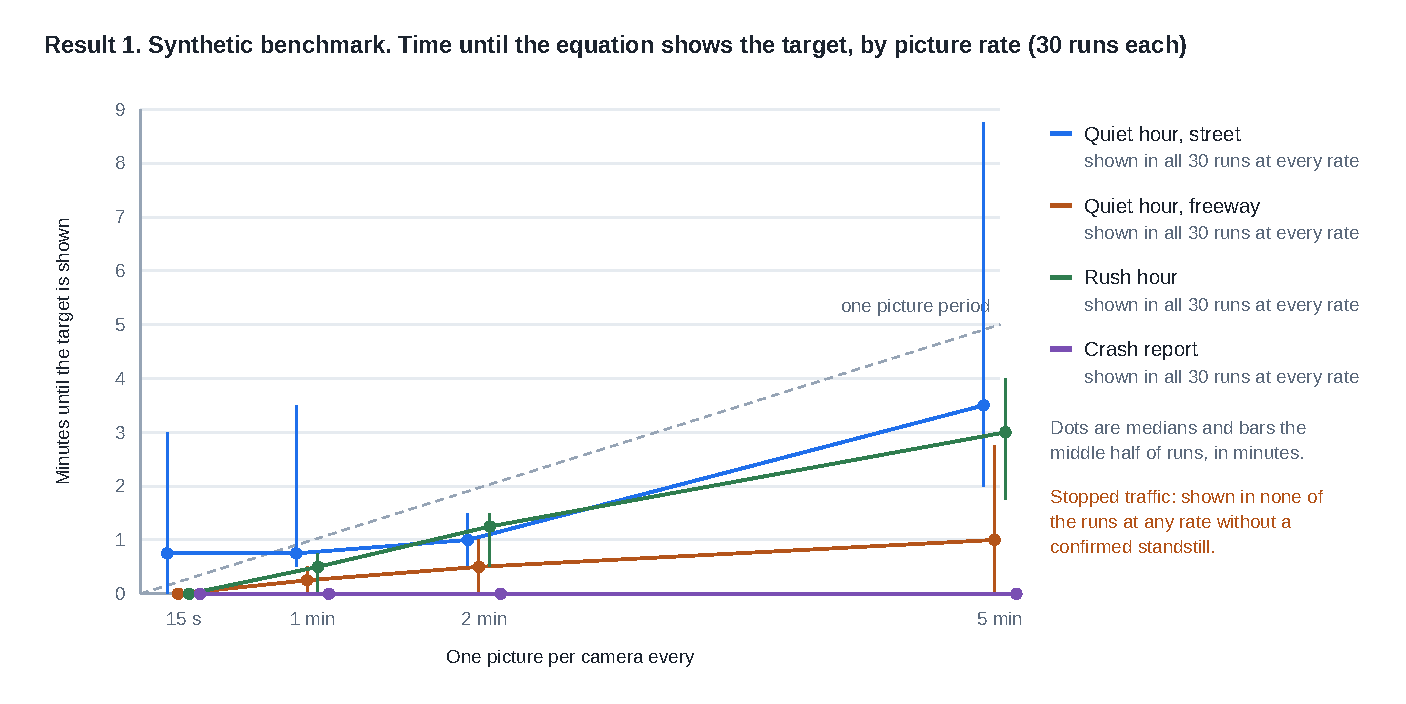
\includegraphics[width=0.9\textwidth]{figures/11-benchmark-picture-rate.pdf}
\caption{Time until the equation shows the target, by picture rate, over 30 runs per cell. Dots are medians and bars span the middle half of runs. The dashed line marks one picture period.}
\label{fig:picturerate}
\end{figure*}

Fig.~\ref{fig:picturerate} repeats the scenarios at one picture every 15 seconds, as sampling a video stream allows, and every 1, 2 and 5 minutes. Slower pictures delay the movement cases roughly in proportion to the picture period, while the crash camera is shown at once at every rate because its floor does not depend on its picture. The largest-difference ranking never showed the rush-hour target at any rate.

The arbiter was run on the stopped-traffic scenario over five seeds and 80 calls. The stopped camera was shown in 0 of 5 runs from frame differences alone and in 1 of 5 runs when the state also carried a vehicle count of 30, the one run in which a single answer crossed the 0.8 gate. On one seed, the standstill probability lay between 0.44 and 0.50 without a count and between 0.75 and 0.78 with it. The threshold was not lowered to pass a synthetic test.

This is a specification test, not evidence that the rules are right. The scenarios, their levels and the noise model were written by the author with the rules in view, and several outcomes follow directly from the definitions. The rush-hour result, for example, holds because anomaly divides by a camera's usual level, which no motion-only ranking does. The benchmark is not selective in what it reports, since every scenario and every seed is reported, including the failures, and it was not tuned to pass, having found four faults in the rules it was written to test. It says nothing about how often these situations occur, how real pictures behave, or whether the equation matches what a person would watch.

\subsection{Live Trace}
\label{sec:trace}
One server watched Columbus, Ohio, from 21:05 to 22:52 Eastern time on 30 September 2026, with a headless browser holding the wall open at $1600 \times 1000$ pixels and the arbiter on. The run was planned for two hours, and the browser was stopped at 22:52 when the host ran short of memory. The city has 80 cameras, all still pictures from ODOT. The decision log recorded 434 rankings of the top 30 cameras, in which 73 distinct cameras appeared.

Six incident records named a logged camera, and all six were ODOT Repairs/Maintenance records. No crash or weather record fell within reach of a Columbus camera during the window. Because every record was then read as road-relevant, these six records and the queues inferred upstream of them held every one of the top 8 places in every ranking, 79\% through an incident floor and 21\% through a queue floor. The wall's limit of 6 held cameras among its prominent tiles left two places to movement, so floors still took 75\% of the top 8. Routine maintenance outranked every unplanned change on the wall for the whole evening, which is the fault behind the planned-work rule of Section~\ref{sec:attention}.

\begin{table}[!t]
\renewcommand{\arraystretch}{1.2}
\caption{Top 8 Places over 434 Rankings in the Columbus Trace}
\label{tab:trace}
\centering
\begin{tabularx}{\columnwidth}{Xcc}
\toprule
\textbf{Top 8 places} & \textbf{As run} & \textbf{Replayed} \\
\midrule
Held by a floor, without the wall's limit & 100\% & 0\% \\
Held by a floor, with the limit of 6 & 75\% & 0\% \\
Won by movement alone, with the limit of 6 & 25\% & 100\% \\
\bottomrule
\end{tabularx}
\end{table}

\begin{figure*}[!t]
\centering
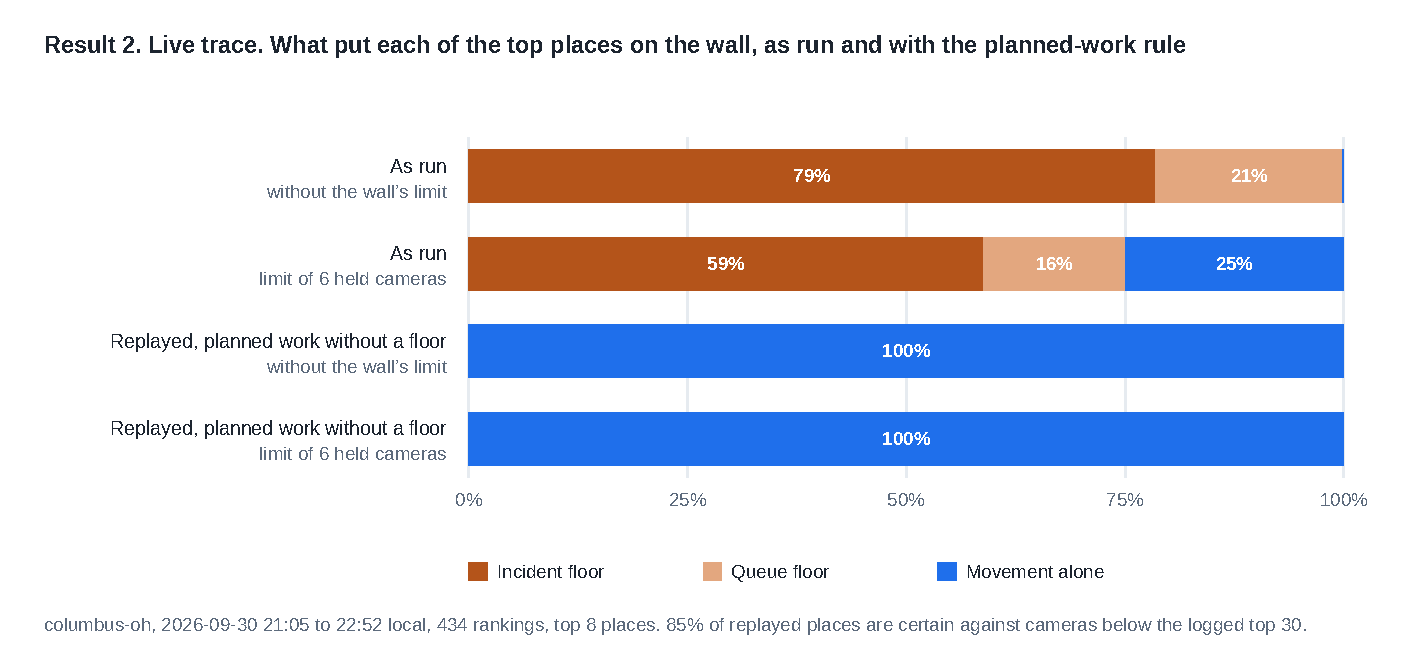
\includegraphics[width=0.9\textwidth]{figures/12-live-trace.pdf}
\caption{What put each of the top 8 places on the Columbus wall, as run and replayed with no floor from planned work, with and without the wall's limit on held cameras.}
\label{fig:trace}
\end{figure*}

Each logged ranking was replayed with no floor from planned work, rescoring every camera from its logged components (Table~\ref{tab:trace} and Fig.~\ref{fig:trace}). The rebuilt score matched the logged score for all 13,020 logged rows before any floor was removed, so the replay differs from the run only in the floors it removes. A camera outside the logged top 30 cannot be rescored, but its score was no higher than the 30th logged camera's and can only have fallen, so a replayed place is certain when its new score is at least that bound. In that sense 85\% of the replayed places are certain. The rule also stops the arbiter from spending calls on planned work, since records that earn no floor are not arbitrated. All 193 incident arbitration calls in the window concerned the six maintenance records.

The stopped-traffic question was asked 19 times, and the standstill probability ranged from 0.31 to 0.45, so no stopped-traffic floor was set. The second look ran 51 times. Its order of the leading cameras agreed with the equation's order with a median Kendall $\tau$ of 0.14, ranging from $-0.50$ to 0.79, and it put the same camera first in 8 of 51 looks. Its answer was confident enough to act on 27 cameras. Against the equation's own score, the look changed on average 0.14 of the top 8 places per ranking as run and 0.42 in the replay, and changed at least one place in 12\% and 40\% of rankings respectively. The floors had left the look little to move. The median call took 221 ms with about 3,000 input tokens.

The server averaged 0.27 requests a second to ODOT over 107 one-minute readings, against a budget of 0.3, with a median of 0.23 and 74 MB an hour. In 35 of the readings the one-minute rate exceeded 0.3, reaching 0.87 apart from the first minute after startup, which reached 1.52. The readings repeat with a period of about 4 minutes, with an autocorrelation of 0.76 at a lag of 4 readings, and the repetition fades over the evening. At startup every camera was first polled within the source's 60-second period, and each then waited its budgeted period of $52 \times 5$ seconds before polling again, so the cameras on screen kept coming due in the same minute. The budget had been applied only through each camera's period, which bounds the average and not the rate. It is now also enforced when each request is sent, and a test that brings 80 cameras into view at once confirms that no minute exceeds the budget.

This is one city on one evening, with no record of what a person would have wanted to see, so it shows what the rules did with real records and real pictures, not whether they did it well. The low agreement between the second look and the equation says the two orders differ, not which is better. The replay is exact for the logged cameras and bounded for the rest, and the replayed wall had no unplanned incident with which to test the floors that remain.

\section{Conclusion}
This paper framed the ranking of public traffic camera feeds on a display wall as an information foraging problem and described rt511, which combines a continuous scorer of anomaly, road size and lexicographic consequence floors with an arbiter consulted only where the arithmetic cannot decide. A synthetic benchmark showed the rules behaving as specified in four of five scripted situations and failing in the fifth, stopped traffic seen only through frame differences, which the arbiter did not resolve from numbers alone. A live trace exposed a fault the benchmark could not, routine maintenance records occupying the wall, and a second in the polling budget, and both were corrected. Whether the ranking directs attention better than any alternative remains untested, and the in-browser preference model and its evaluation mode exist to make that test possible.

\bibliographystyle{IEEEtran}
\bibliography{references}

\end{document}